\documentclass[aspectratio=169]{beamer}

% ---------- ENCODING & FONTS ----------
\usepackage[utf8]{inputenc}
\usepackage[T1]{fontenc}

% ---------- THEME & LOOK ----------
\usetheme{Madrid}
\usecolortheme{seahorse}
\usefonttheme{professionalfonts}
\setbeamertemplate{navigation symbols}{}
\setbeamercovered{transparent}
\setbeamertemplate{itemize items}[circle]
\setbeamertemplate{enumerate items}[default]
\setlength{\parskip}{0.25em}

% ---------- COLORS ----------
\usepackage{xcolor}
\definecolor{accent}{RGB}{0,92,184}
\definecolor{soft}{RGB}{233,244,255}
\setbeamercolor{structure}{fg=accent}
\setbeamercolor{title}{fg=white,bg=accent}
\setbeamercolor{frametitle}{fg=accent}
\setbeamercolor{block title}{bg=accent!12,fg=accent}
\setbeamercolor{block body}{bg=soft}

% ---------- PACKAGES ----------
\usepackage{booktabs}
\usepackage{amsmath, amssymb}
\usepackage{array}
\usepackage{hyperref}
\hypersetup{colorlinks=true,linkcolor=accent,urlcolor=accent}

% ---------- SAFE FALLBACK FOR TRANSITIONS ----------
\makeatletter
\@ifundefined{transfade}{\newcommand{\transfade}[1][]{}}{}
\makeatother

% ---------- PLACEHOLDER BOX (compile-safe; no images required) ----------
\newcommand{\placeholderbox}[2][0.82\linewidth]{%
  \begin{center}
    \fbox{\begin{minipage}[c][0.46\textheight][c]{#1}
      \centering \vspace{0.25em}
      \textbf{#2}\\[0.6em]
      \emph{Insert figure/diagram here later.}
    \end{minipage}}
  \end{center}
}

% ---------- TITLE ----------
\title{\textbf{Discrimination and Male -- Female Earnings Differentials \vspace{.5cm}\\  }}
\subtitle{ {\large ECON 300 - Labour Economics}}
%\institute{UNBC}
\author{Muhebullah Karimzada}

\date{Winter 2026}



\begin{document}

% ============================================================
% TITLE
% ============================================================
\begin{frame}[plain]
  \titlepage
\end{frame}

% ============================================================
\section{Learning Objectives \& Questions}
% ============================================================

\begin{frame}{Learning Objectives}
\transfade
\begin{itemize}[<+->]
  \item Describe the factors giving rise to male--female pay gaps and the role of discrimination.
  \item Outline methodologies used to estimate discriminatory pay gaps and their challenges.
  \item Explain how discriminatory gaps can persist even with competitive pressures.
  \item Discuss pros and cons of policy initiatives to combat discrimination.
  \item Explain the evolution of the gender pay gap and the mechanics of pay equity.
\end{itemize}
\end{frame}

\begin{frame}{Main Questions}
\transfade
\begin{itemize}[<+->]
  \item How can equally productive men and women be paid different wages in competitive markets?
  \item Will competitive forces dissipate discrimination?
  \item How do we measure discrimination credibly in the data?
  \item How much discrimination exists in Canada? What about other groups?
  \item Which policies have been adopted, and which are effective?
\end{itemize}
\end{frame}

% ============================================================
\section{Theories and Evidence}
% ============================================================

\begin{frame}{What is Labour-Market Discrimination?}
\transfade
\begin{itemize}[<+->]
  \item Unequal treatment of groups with the same productivity (or productivity-related traits).
  \item \textbf{Who can discriminate?}
    \begin{itemize}[<+->]
      \item \alert{Employers}: wages, hiring, promotions
      \item \alert{Co-workers}: prejudice, misinformation, job-security concerns
      \item \alert{Customers}: discriminatory preferences
    \end{itemize}
\end{itemize}
\end{frame}

\begin{frame}{Theory Map}
\transfade
\begin{itemize}[<+->]
  \item \textbf{Demand theories}
  \item \textbf{Supply theories}
  \item \textbf{Noncompetitive theories}
  \item \textbf{Queuing} and efficiency-wage considerations
\end{itemize}
\end{frame}

\begin{frame}{Demand Theories of Discrimination}
\transfade
\begin{itemize}[<+->]
  \item Lower \alert{demand} for female labour \(\Rightarrow\) lower wages and employment.
  \item Possible channels:
    \begin{itemize}[<+->]
      \item Underestimation of female productivity
      \item Statistical discrimination / signalling stories
    \end{itemize}
\end{itemize}
\end{frame}

\begin{frame}{Supply Theories of Discrimination}
\transfade
\begin{itemize}[<+->]
  \item Increased \alert{supply} of female labour depresses wages if productivity or matching suffers.
  \item \textbf{Crowding hypothesis:} Segregation into “female-type” jobs \(\Rightarrow\) excess supply \(\Rightarrow\) lower MRP and wages.
  \item \textbf{Dual labour market:} Men in core, women in secondary sector \(\Rightarrow\) lower wages in secondary market.
\end{itemize}
\end{frame}

\begin{frame}{Noncompetitive \& Queuing Theories}
\transfade
\begin{itemize}[<+->]
  \item \textbf{Noncompetitive:} Adjustment costs and imperfect information can sustain gaps.
  \item \textbf{Queuing/Efficiency wages:} Firms pay above-competitive wages to reduce turnover and improve morale, creating queues that can interact with group differences.
\end{itemize}
\end{frame}

\begin{frame}{Productivity Differences: Choice or Discrimination?}
\transfade
\begin{itemize}[<+->]
  \item Differences in acquired human capital may reflect:
    \begin{itemize}[<+->]
      \item Shorter expected labour-force attachment
      \item Higher turnover or absenteeism
      \item Household and caregiving responsibilities
    \end{itemize}
\end{itemize}
\end{frame}

% ============================================================
\section{Measuring Discrimination}
% ============================================================

\begin{frame}{Setup: Oaxaca(-Blinder) Decomposition}
\transfade
\small
Let \( \ln W = X\beta + \varepsilon \), estimated separately for men (m) and women (f).
\[
\overline{\ln W}_m - \overline{\ln W}_f
= (\overline{X}_m - \overline{X}_f)^\top \hat{\beta}_m
\;+\; \overline{X}_f^{\top}(\hat{\beta}_m - \hat{\beta}_f)
\]
\begin{itemize}[<+->]
  \item First term: part “explained” by differences in characteristics (\(\overline{X}\)).
  \item Second term: \alert{coefficient effect} (“unexplained”/often attributed to discrimination).
  \item Reference structure can be male, female, or pooled (affects magnitudes).
\end{itemize}
\end{frame}

\begin{frame}{Figure 12.1: Graphical Illustration of the Oaxaca Decomposition}
\centering
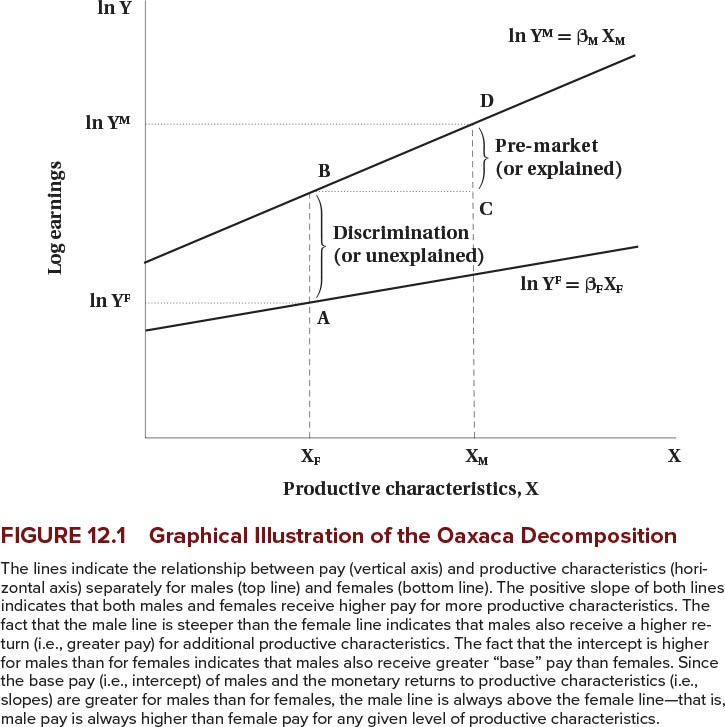
\includegraphics[width=0.7\linewidth]{ben54842_1201}
\end{frame}

\begin{frame}{Worked Example: Analyzing the Determinants of Earnings}
\transfade
\small
Estimated earnings equations:
\[
\begin{aligned}
\text{Men:}\quad & \ln W_m = 0.40 + 0.07\,S + 0.06\,\text{EXP} + 0.05\,\text{Married} + 0.01\,\text{Children} \\
\text{Women:}\quad & \ln W_f = 0.01 + 0.10\,S + 0.04\,\text{EXP} - 0.02\,\text{Married} - 0.05\,\text{Children}
\end{aligned}
\]
Group means:
\[
\overline{X}_m=(S{=}14, \text{EXP}{=}10, M{=}0.5, C{=}0.6),\;
\overline{X}_f=(S{=}15, \text{EXP}{=}7, M{=}0.5, C{=}0.6).
\]
\end{frame}

\begin{frame}{Worked Example: Predicted Values and Raw Gap}
\transfade
\small
\[
\begin{aligned}
E(\ln W_m) &= 0.40 + 0.07(14) + 0.06(10) + 0.05(0.5) + 0.01(0.6) = \mathbf{2.01} \\
E(\ln W_f) &= 0.01 + 0.10(15) + 0.04(7) - 0.02(0.5) - 0.05(0.6) = \mathbf{1.75}
\end{aligned}
\]
Raw ratio (female to male):
\[
\frac{E(\ln W_f)}{E(\ln W_m)} = \frac{1.75}{2.01} \approx \mathbf{0.87}.
\]
\end{frame}

\begin{frame}{Worked Example: Counterfactual Pay Structures}
\transfade
\small
Female characteristics, \textbf{male} coefficients:
\[
\ln W_f^{\ast} = 0.40 + 0.07(15) + 0.06(7) + 0.05(0.5) + 0.01(0.6) = \mathbf{1.90}
\]
Male characteristics, \textbf{female} coefficients:
\[
\ln W_m^{\ast} = 0.01 + 0.10(14) + 0.04(10) - 0.02(0.5) - 0.05(0.6) = \mathbf{1.77}
\]
Implications:
\[
\ln W_f^{\ast} - E(\ln W_m) = {1.90} - {2.01} = \mathbf{-0.11},\quad
E(\ln W_f) - \ln W_m^{\ast} = {1.75} - {1.77} = \mathbf{-0.02}.
\]
\end{frame}

% ============================================================
\section{Additional Evidence}
% ============================================================

\begin{frame}{Additional Evidence on Male--Female Pay Differentials}
\transfade
\begin{itemize}[<+->]
  \item Studies examine wage, sex, institutional, and household discrimination channels.
  \item Average female earnings often reported at \(\sim 60\)–\(65\%\) of male earnings in some datasets/periods, reflecting barriers (e.g., glass ceilings) and composition effects.
  \item Key question: \alert{What would women earn if they were men?} Use counterfactuals holding productive traits fixed.
\end{itemize}
\end{frame}

\begin{frame}{Empirical Evidence for Other Groups}
\transfade
\scriptsize
\textbf{Table 12.1: Ethnic Wage Differentials, Various Groups Born in Canada or United States}
\medskip

\begin{tabular}{lccccc}
\toprule
 & \textbf{Black} & \textbf{South Asian\textsuperscript{a}} & \textbf{Southeast Asian\textsuperscript{b}} & \textbf{Chinese} & \textbf{Aboriginal} \\
\midrule
\multicolumn{6}{l}{\textit{Canada}} \\
Total gap & 0.293 & 0.536 & $-0.022$ & 0.193 & 0.179 \\
``Discrimination'' & 0.171 & 0.222 & 0.023 & 0.058 & 0.091 \\
\addlinespace[0.25em]
\multicolumn{6}{l}{\textit{United States}} \\
Total gap & 0.328 & 0.176 & $-0.079$ & $-0.205$ & 0.304 \\
``Discrimination'' & 0.123 & 0.055 & $-0.007$ & $-0.047$ & 0.136 \\
\bottomrule
\end{tabular}

\medskip
\scriptsize \textit{Notes:} Column headers match the original table; \textsuperscript{a}South Asian, \textsuperscript{b}Southeast Asian.
\end{frame}

% ============================================================
\section{Policies to Combat Discrimination}
% ============================================================

\begin{frame}{Policy Toolkit}
\transfade
\begin{itemize}[<+->]
  \item \textbf{Conventional equal pay:} Same job, same establishment.
  \item \textbf{Equal value / Pay equity / Comparable worth:} Job evaluation to compare across predominantly male vs.\ female jobs.
  \item \textbf{Equal employment opportunity (EEO):} Recruitment, hiring, promotion protections.
  \item \textbf{Affirmative action / Employment equity:} Targeted plans for designated groups.
  \item \textbf{Facilitating policies:} Childcare, family-friendly practices to broaden choices.
\end{itemize}
\end{frame}

\begin{frame}{Equal Pay and Pay Equity}
\transfade
\begin{itemize}[<+->]
  \item \textbf{Equal pay legislation:} Equal pay for equal \emph{value} within the same establishment; job evaluation must be gender-bias-free.
  \item Scope: All Canadian jurisdictions except Alberta.
\end{itemize}
\end{frame}

\begin{frame}{Comparable Worth: Design Features}
\transfade
\begin{itemize}[<+->]
  \item Define gender predominance and choose job-evaluation procedure.
  \item Specify adjustment procedures and possible exemptions.
  \item Scope can be large (cross-occupation comparisons), but enforcement and complaints may be limited in practice.
\end{itemize}
\end{frame}

\begin{frame}{EEO and Employment Equity}
\transfade
\begin{itemize}[<+->]
  \item EEO: Prevents discrimination in recruiting/hiring/promotion; can raise female employment and wages; complements equal pay.
  \item Employment equity: Federal jurisdiction; \(\sim 10\%\) of labour force; designated groups include women, visible minorities, persons with disabilities, and Aboriginal people.
\end{itemize}
\end{frame}

\begin{frame}{Overall Impact}
\transfade
\begin{itemize}[<+->]
  \item \textbf{Equal pay / EEO:} Mixed evidence on broad wage-gap closures.
  \item \textbf{Comparable worth:} Evidence of gap reductions where implemented.
  \item \textbf{Bottom line:} Impacts exist but can be limited by scope, design, and enforcement.
\end{itemize}
\end{frame}

% ============================================================
\section{Summary}
% ============================================================

\begin{frame}{Summary}
\transfade
\begin{itemize}[<+->]
  \item Defined discrimination, reviewed demand/supply/noncompetitive/queuing theories.
  \item Implemented Oaxaca-type decompositions to separate endowments vs.\ coefficients.
  \item Reviewed evidence on gender and other-group differentials, including exact table values.
  \item Assessed policy tools: equal pay, pay equity, EEO, employment equity, and facilitating policies.
\end{itemize}
\end{frame}

\begin{frame}
\centering
\Huge{\textbf{Thank You!}} \\

\end{frame}

\end{document}
